\section{What has been achieved in CY2014 and Plan for CY2015}


\paragraph{Pulsar II:  Pulsar IIb has been successfully tested with excellent results}

Leveraging the experience we gained through designing, building and testing the Pulsar IIa board, we have successfully designed and tested the next generation board, the Pulsar IIb (as shown in Figure~\ref{fig:ProcBlade}).
Most of the hardware design work for the Puslar II has been done in FY2014~\cite{bib:PulsarII}, including the successful design~\cite{bib:PulsarII-results}~\cite{bib:PulsarII-weblink} and testing of Pulsar IIb and its related hardware. 
The details of most recent progress report on Pulsar IIb can be found here~\cite{bib:joint-meeting}.

  The Pulsar IIb design replaces the two Kintex K325T devices with a single large Virtex-7 FPGA.  The GTH transceiver count has increased up to 80 channels, providing a significant bandwidth increase to the RTM, Fabric and Mezzanine cards. The Pulsar IIa design was originally motivated by Atlas FTK needs, but the Pulsar IIb is designed to meet the challenging requirements of CMS L1 tracking trigger demonstration. As such, the performance of the actual Pulsar IIb far exceeds the original FTK requirements. 
This includes the 80 GTH high speed (10Gbps) birectional communication channels from the Virtex-7 FPGA with challenging layout work for large ATCA board, the capability to interface with CMS TTC/FMC card, the capability to distribute TTC clock signals over the backplane so all Pulsar II based crates can run in sync with each other (important for L1 trigger applications), as well as the capability to be compatible with CMS IPBus protocol. The Pulsar IIb, as it is designed, can be used as the workhorse for the Vertical Slice Demonstration system for CMS L1 tracking trigger. The next milestone will be the full crate level testing with Pulsar IIb. Most of the Pulsar IIb design work is supported by non-CMS funds.

\begin{figure}[ht!]
\centering
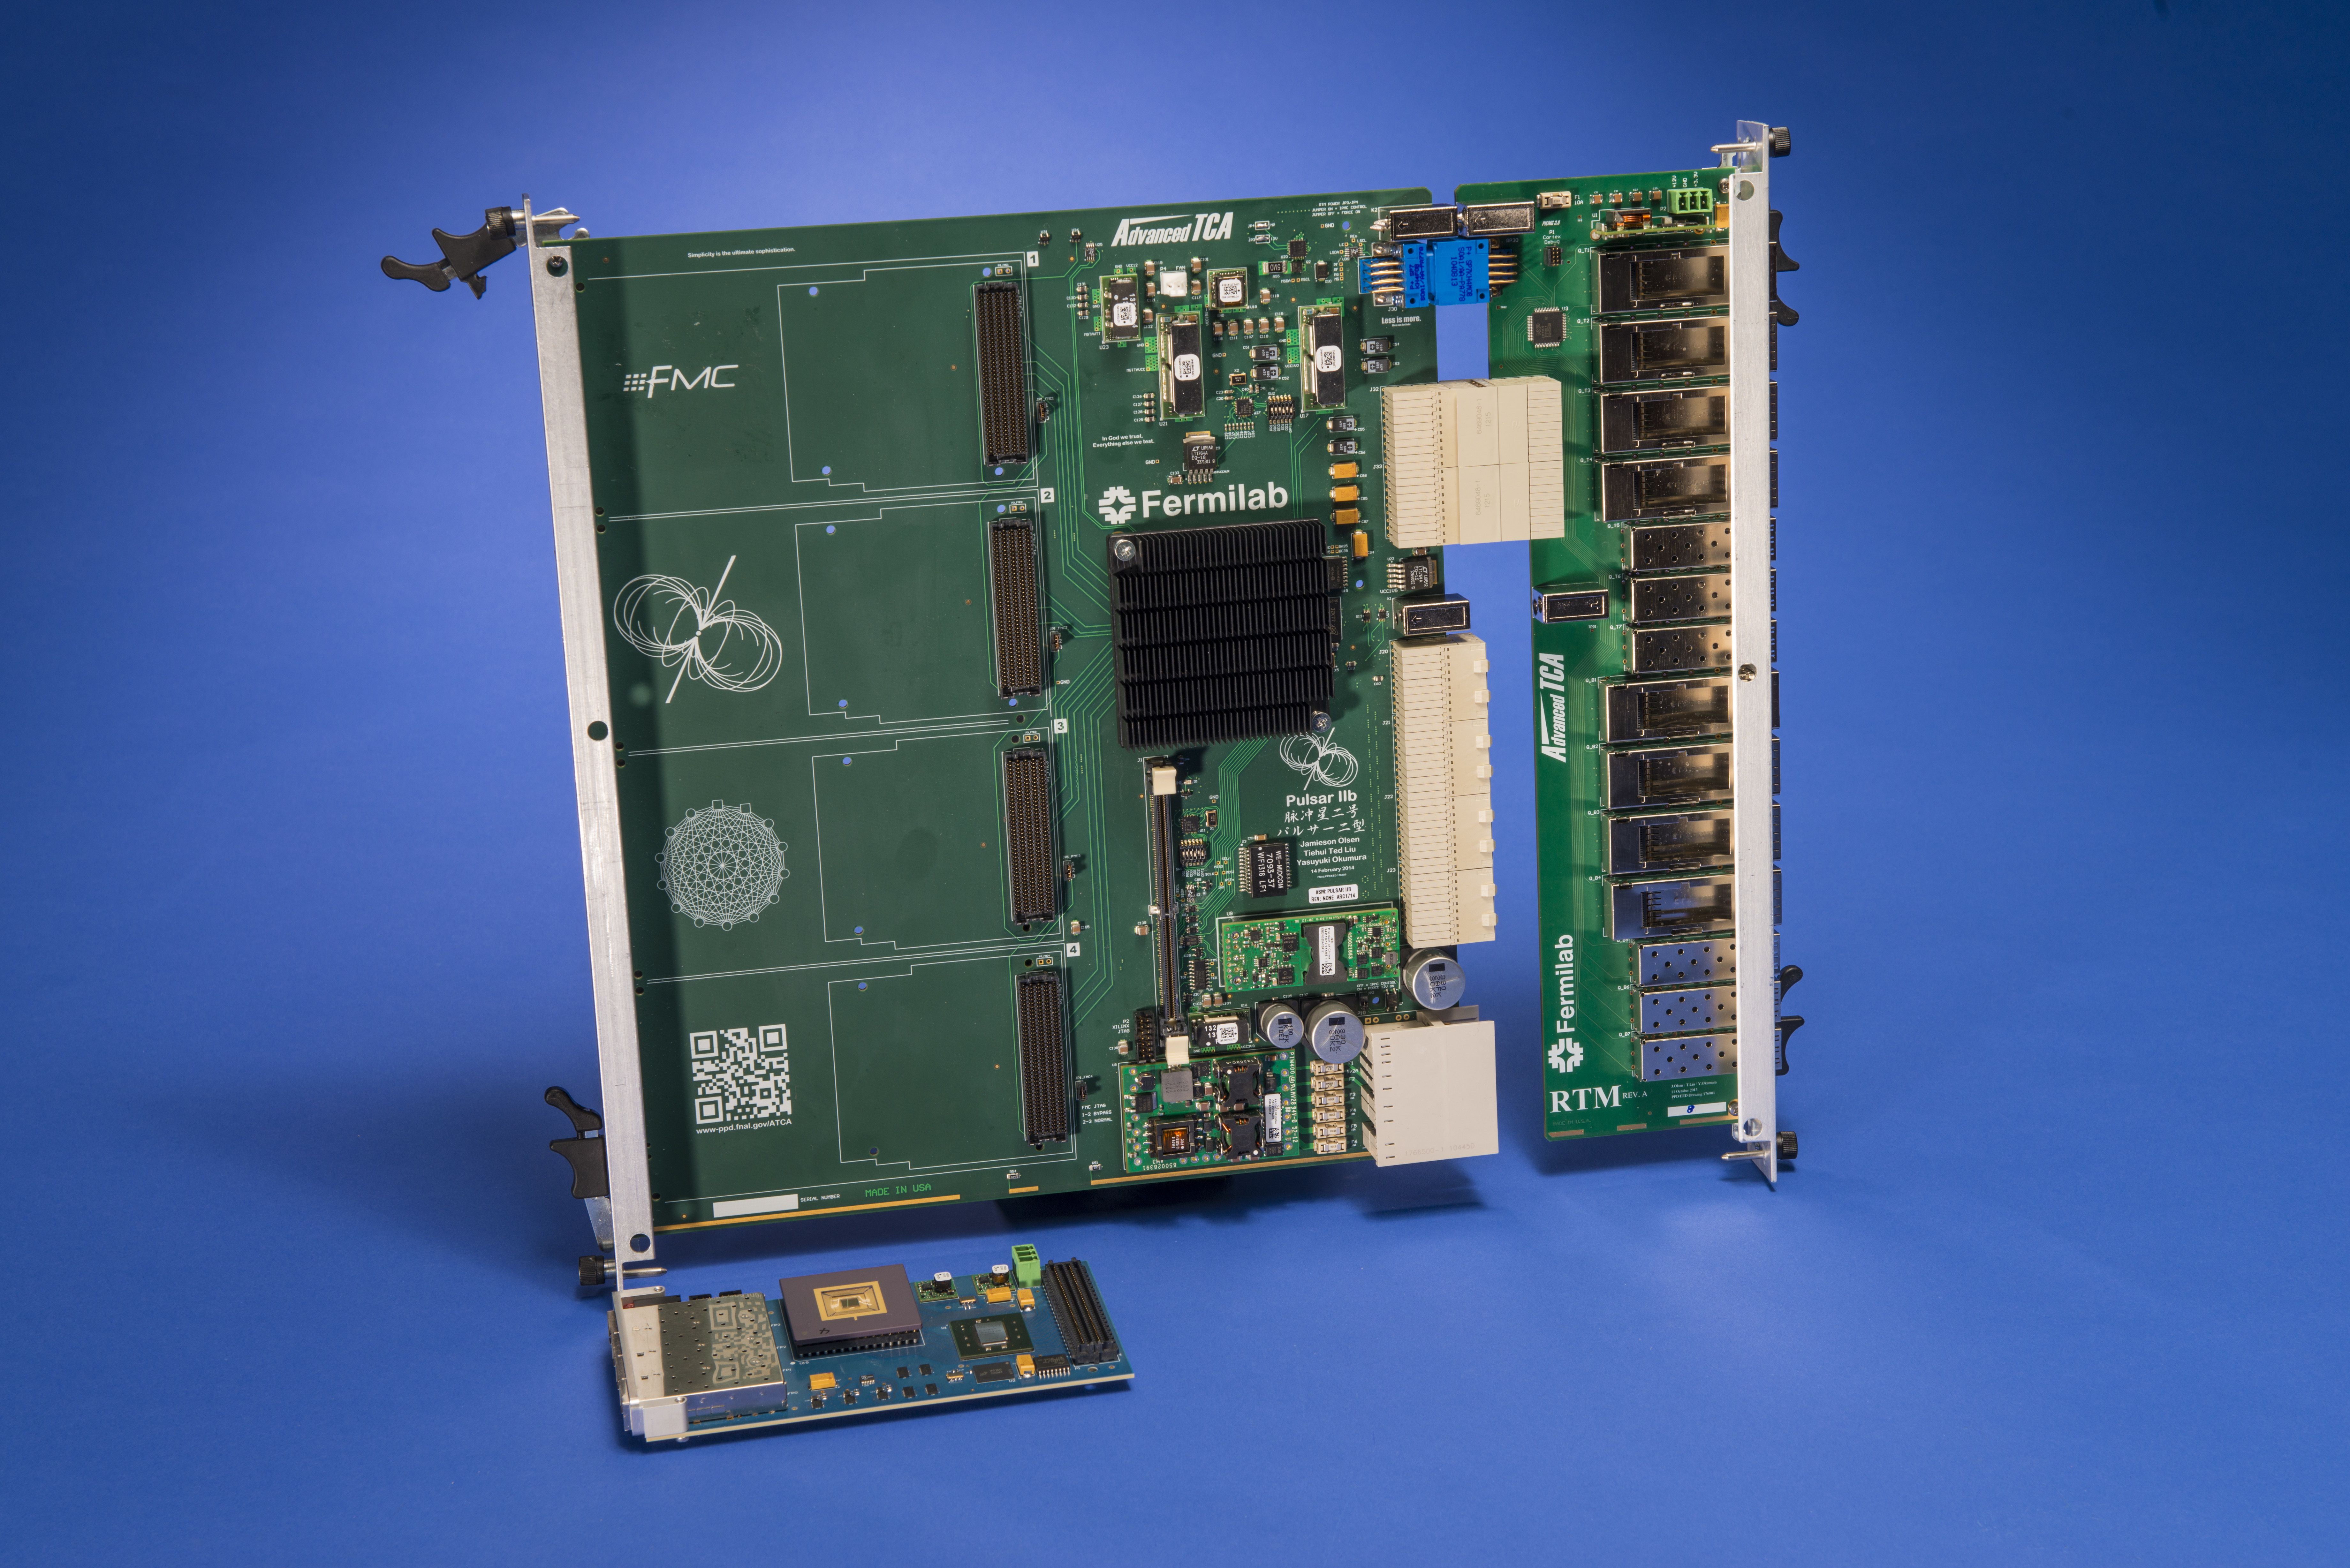
\includegraphics[width=0.8\columnwidth]{Plots/Pulsar2b-photo-compressed}
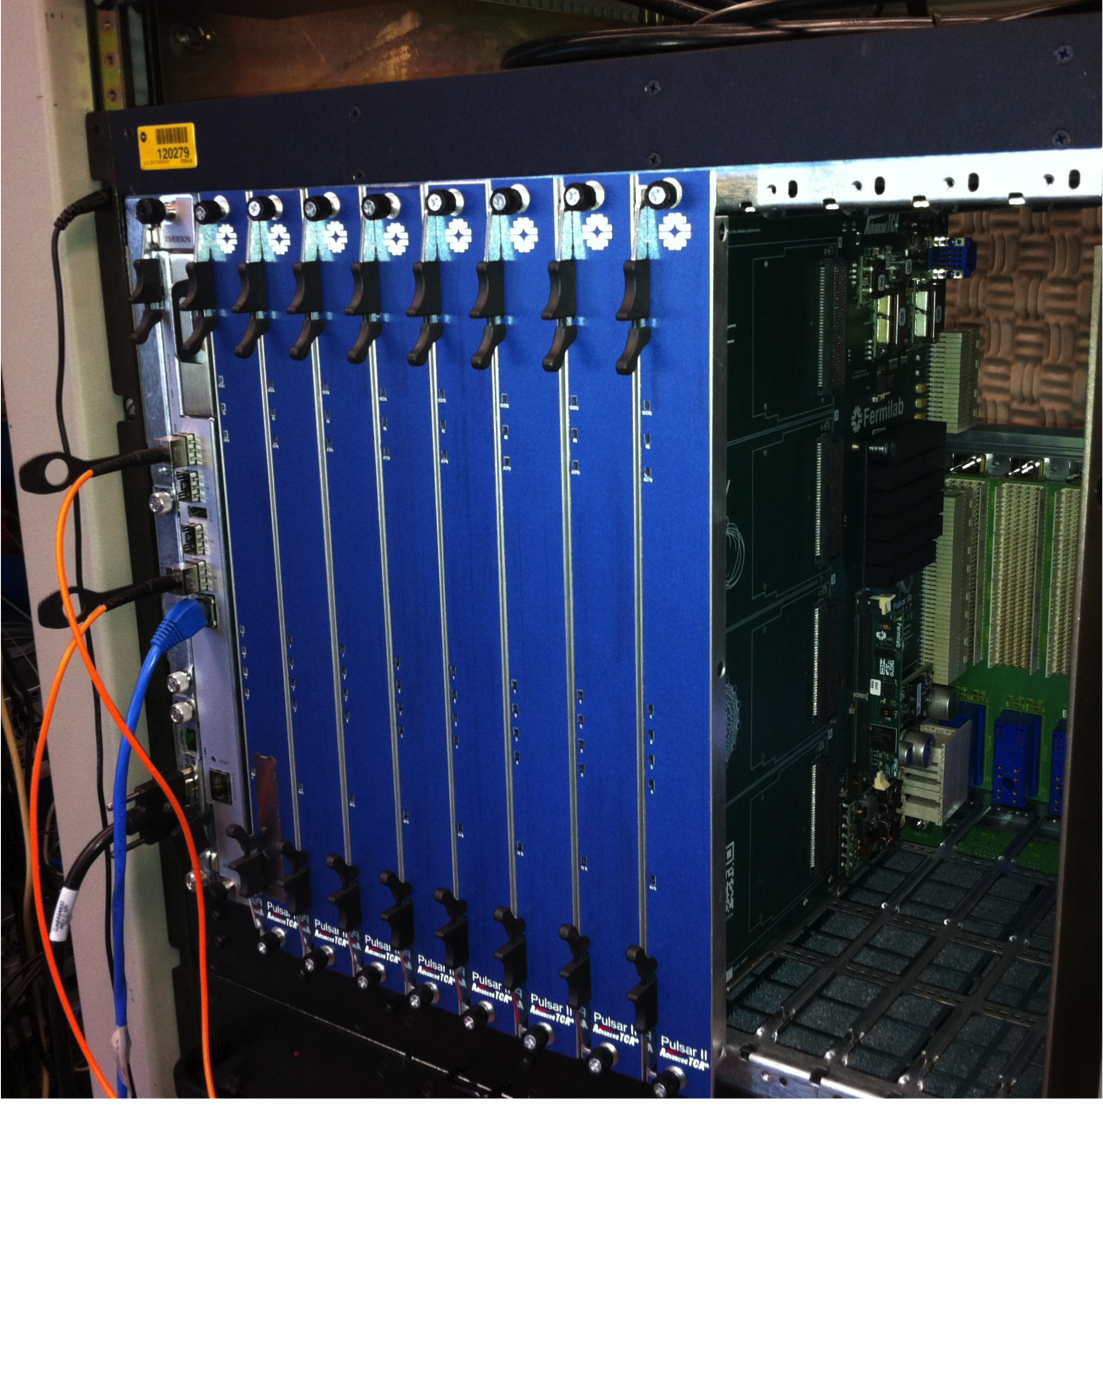
\includegraphics[width=0.2\columnwidth]{Plots/PuslarIIb-crate}
\caption{Top: The Pulsar IIb~\cite{bib:PulsarII}~\cite{bib:PulsarII-weblink} with its prototype mezzanine card.
Bottom: Pulsar IIb crate.}
\label{fig:ProcBlade}
\end{figure}


\paragraph{ATCA 40G high performance full-mesh backplane evaluation using Pulsar IIb}

Few vendors worldwide can produce ATCA shelves with a 40G high performance full-mesh backplane.
Because the Pulsar 2b fabric full-mesh performance is excellent (tested to 10 Gbps), two Pulsar IIbs are being used to evaluate the
performance of 40G ATCA crate from different vendors. The vendors are very interested in our capability to test their backplanes, and they are offering us free ATCA shelves for short term (2-3 months) evaluation purposes.  We have been testing three so far, with another due to arrive soon. Our testing results show that not all 40G full-mesh backplanes are created equal, and we will pick the best one among them.


\paragraph{Pulsar IIb new RTM, Mini-backplane, and IPMC card}

A new RTM design has been finished and submitted recently. This version has increased the channel counts from 38 to 40 (all bidirectional) to be fully compatible with the Pulsar IIb, and has improved high speed signal routing and power regulation and distribution. This version allows eight PulsarIIb boards to sink or source 320 optical links (or modules), the number of modules/fibers targeted for one trigger tower. This RTM revision work is supported by USCMS funding.

A new Mini-Backplane has been developed to loop back all fabric interface channels for high speed (10 Gbps) Pulsar IIb self testing. It also has Base Interface Ethernet ports brought out to RJ45 and SFP+, which enables single board testing on the bench top. The new mini-backplanes have been used extensively during Pulsar IIb testing, and have proven to be highly valuable.  This mini-backplane revision work is supported by USCMS funding.


An IPMC (Intelligent Platform Management Controller) mezzanine card has been developed at Fermilab. 
An IPMC is required for all ATCA boards.  The controller talks to the shelf manager to coordinate hot swap, e-keying, and to monitor various board sensors. The FNAL IPMC card has successfully powered up the Pulsar2b and RTM, and it is now part of the Pulsar IIb. This IPMC work is supported by USCMS funding.

\begin{figure}[ht!]
\centering
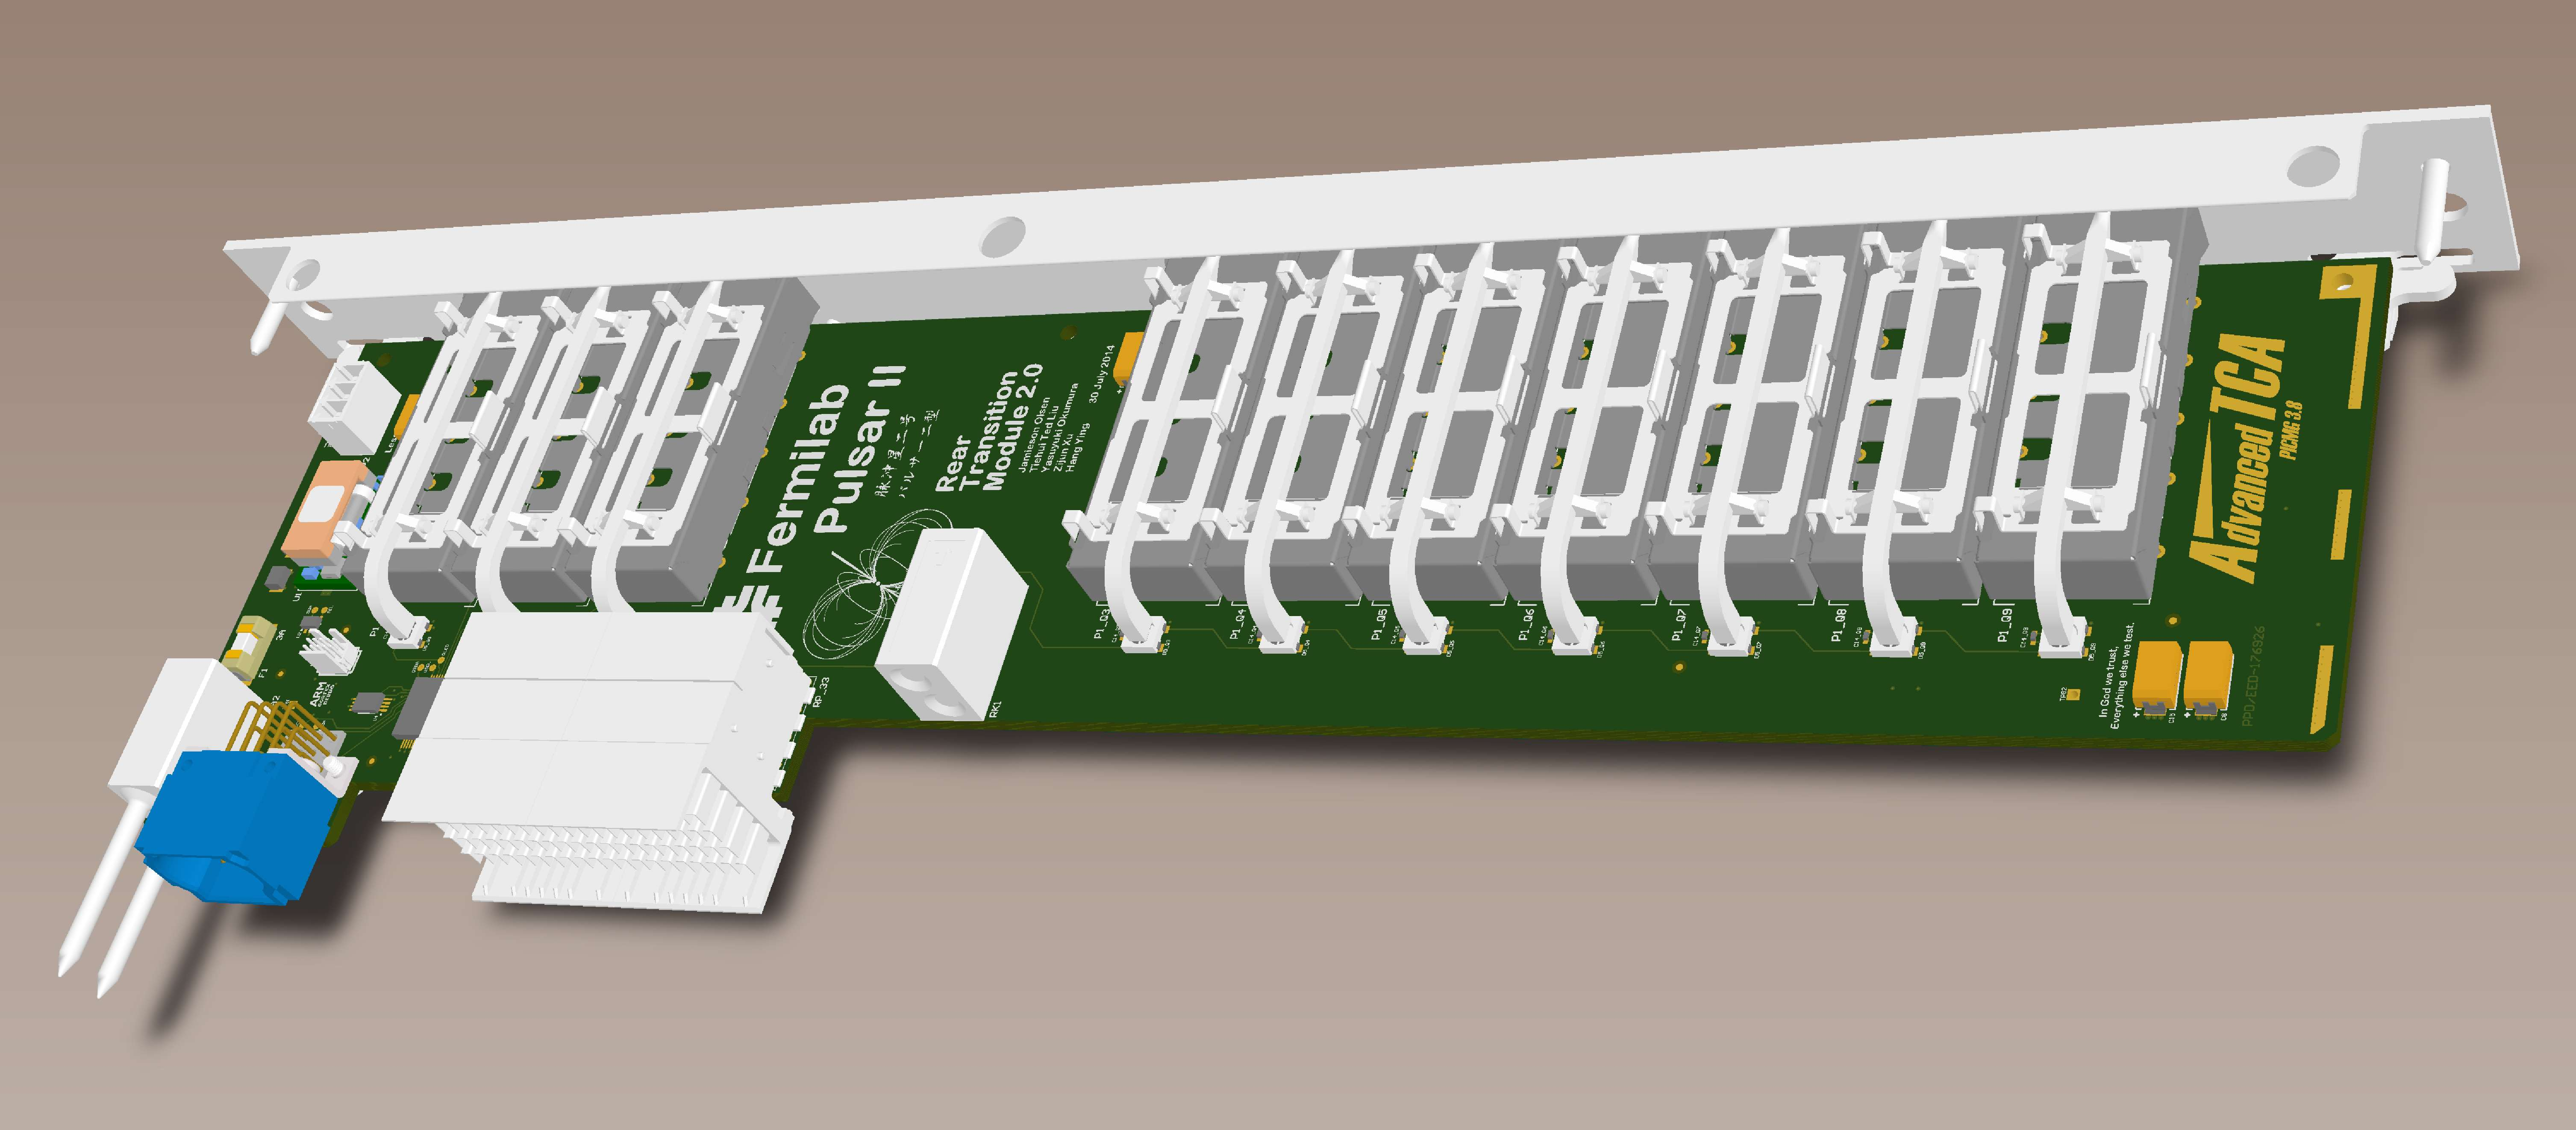
\includegraphics[width=0.8\columnwidth]{Plots/RTM_v20}
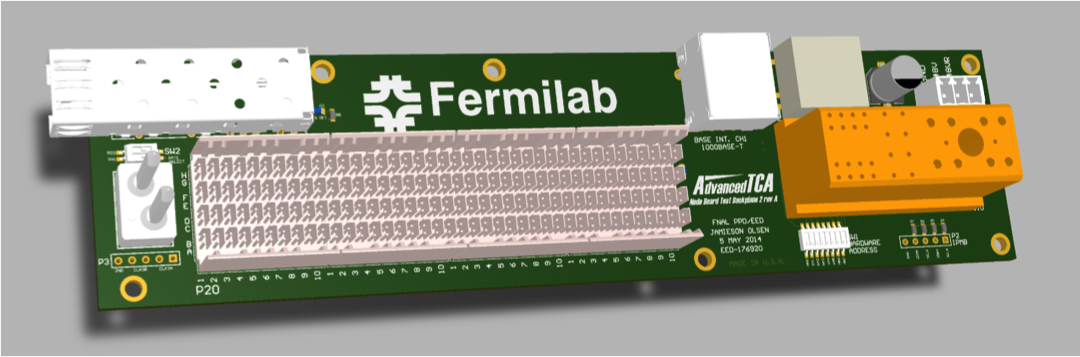
\includegraphics[width=0.4\columnwidth]{Plots/FNAL-mini-backplane.png}
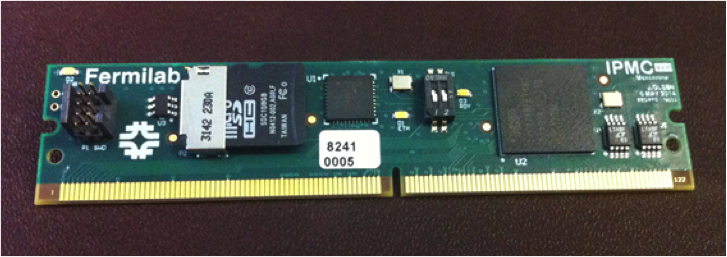
\includegraphics[width=0.4\columnwidth]{Plots/FNAL-IPMC.png}
\caption{Top: The Pulsar IIb new RTM design, just submitted. Bottom Left: Pulsar IIb new mini-backplane; Bottom Right: Pulsar IIb FNAL IPMC card.}
\label{fig:PulsarIIb-RTM}
\end{figure}



\paragraph{Next versions of Pattern Recognition Mezzanine card design in progress}

This is the core pattern recognition engine, and is being designed to host the protoVIPRAM-L1CMS chips for pattern recognition, and the latest Xilinx Ultra Scale FPGAs for high performance track fitting. This design is now in progress and will be one of the two major engineering efforts in FY2015 (the other being the protoVIPRAM-L1CMS chip design). 

Track reconstruction typically consists of two steps: pattern recognition followed by track fitting. Pattern recognition involves choosing, among all the hits present in the detector, those hits that were potentially caused by the same particle. The Associative Memory (AM) approach~\cite{bib:Rist-89} solves the combinatorial problem (due to high occupancy) inherent in this kind of pattern recognition task by employing a massively parallel architecture to simultaneously compare each detector hit to a large number of pre-calculated geometrical patterns. The AM solves the pattern recognition problem in essentially zero time, and only pass the hits of interests to track fitting stage therefore making the downstream task easier and faster.

The pattern recongition stage produces a set of hits of interest. Track fitting involves extracting track parameters from the
coordinates of these hits.  As soon as hits have been loaded in the AM, found patterns (or fired roads) are ready to be output and processed (fit) with fast FPGAs. Because each pattern corresponds to a very narrow "road” through the detector, the usual helical fit can be considerably simplified by using a pre-calculated set of parameter values for the center of the road.  Corrections are then applied as a linear function of the actual hit positions in each layer. The hits or stubs of interest within each road are combined to form tracks this way. Track helix parameters and χ2 can be extracted from the linear equations in the local silicon hit coordinates. It has been shown (by FTK and SVT) that very good performance (in terms of the resolution of the linear fit) can be achieved this way using modern FPGA DSPs. Note that the Xilinx Ultra Scale FPGAs are known for their enhanced DSP capacity, making them a suitable choice forthe pattern recognition mezzanine card.

Both the pattern recognition and track fitting stages will be implemented on the pattern recognition mezzanine card, making it the most important core pattern recogniton engine of the entire L1 tracking trigger system. The main challenge of this work is likely the firmware work due to the low latency requirement for CMS L1 tracking trigger. 

\begin{figure}[ht!]
\centering

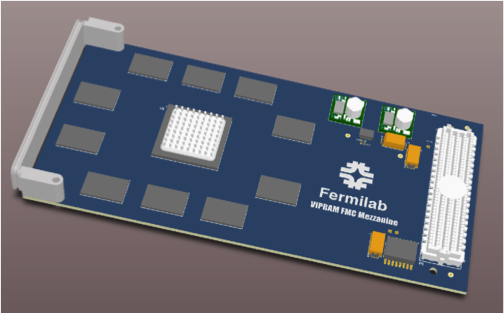
\includegraphics[width=0.6\columnwidth]{Plots/mezzanine-concept.png}
\caption{The pattern recognition mezzanine card conceptual design (compatible with Pulsar II). The new mezznine card being designed is double width mezzanine.}
\label{fig:mezzanine-concept}
\end{figure}


\paragraph{VIPRAM R\&D: ProtoVIPRAM 2D chip has been successfully tested}

The numerous advantages of an Associative Memory-based track trigger are well established.  Its primary limitations lie in pattern density and in readout speed for Level 1 trigger applications.  A secondary challenge is to minimize power consumption.  Vertical Integration is an emerging technology which offers dramatic improvements in all these areas.  The overall objective of the VIPRAM project at this point is to make steady progress towards a final solution.  This requires a strategic approach to architecture and layout that permits near term solutions in classical VLSI technology and long term solutions in aggressive Vertical Integration. 

From the beginning, our design methodology has been to develop concepts and circuitry in 2D to confirm functionality as economically as possible and then to translate, where necessary, those ideas into 3D.  The first step taken by the VIPRAM Project was the development of a 2D prototype (protoVIPRAM1) in which the associative memory building blocks were laid out as if this was a 3D design.  Room was left for as yet non-existent Through Silicon Vias and routing was performed to avoid these areas.  
%In protoVIPRAM1, there are four independent but identical CAM cells for each Control cell arranged into a unit called a protoLeg.  Each protoLeg %contains all the memory, comparison circuitry and evaluation logic necessary to perform the pattern recognition algorithm for one complete 4-layer %road.  protoVIPRAM1 is an array of 32 by 128 protoLeg cells.  
The readout circuitry is deliberately simplified to allow direct performance studies of the CAM and Control cells.  The protoVIPRAM1 was designed and fabricated in a 130nm Low Power CMOS process.  The design was thoroughly simulated at all levels before submission and the teststand was fully ready before the chips arrived. In fact, we were able to correctly observe found patterns the day after the first prototype chip became available for testing. 

The first prototypes of the protoVIPRAM verifies the CAM and majority logic designs for future use in more application specific chips. The testing results match the simulation studies and show that these building blocks are ready for 3D stacking.  The results have been presented at the Front-end electronics workshop (FEE 2014).  More detailed testing results of the prototype will be presented at TWEPP 2014. This work is supported by DOE CDRD funds.


\begin{figure}[ht!]
\centering
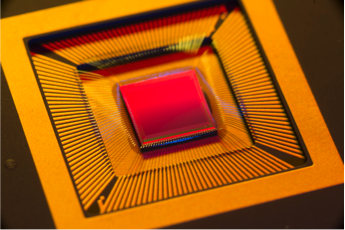
\includegraphics[width=0.3\columnwidth]{Plots/ProtoVIPRAM-photo.png}
\includegraphics[width=0.6\columnwidth]{Plots/ProtoVIPRAM-mezzanine.png}
\caption{The protoVIPRAM and its testing mezzanine card (compatible with Pulsar II). This prototype mezzanine has been used extensively in FY 2014 to test the protoVIPRAM chips.}
\label{fig:ProtoVIPRAM}
\end{figure}


\paragraph{VIPRAM R\&D: Next versions of ProtoVIPRAM design in progress}

The VIPRAM approach has, from the beginning, attempted to increase pattern density and decrease power density through Vertical Integration.   To mitigate issues implicit in adopting an emerging technology, a flexible architecture has been developed that can be implemented in either conventional or Vertically Integrated VLSI.  This allows us to bring the system interface to maturity at an early stage while, at the same time, making steady progress towards the final VIPRAM solution.  This is particularly important for Level 1 Tracking Trigger applications. The protoVIPRAM1 is the first step to developing the next generation AM chips for L1 applications. 
The next two steps will be performed in parallel. We now have two designs in progress:  protoVIPRAM3D and protoVIPRAM-L1CMS.

The protoVIPRAM3D takes the circuitry designed in protoVIPRAM1 and vertically integrates it.  The Control cells are moved onto a Control Tier and the CAM cells become a CAM Tier.  Since the basic building blocks are already fully tested in 2D, what we will be testing with protoVIPRAM3D is the 3D design and process. The chip interface will be kept the same as the protoVIPRAM1, so that the testing can be done in the same way, allowing us to compare directly the 3D version performance with that of the 2D. This work is supported by DOE CDRD funds.

The protoVIPRAM-L1CMS for CMS, on the other hand, attempts to improve the data input and readout speed of the associative memory chips and bring the system-level interface to maturity using conventional 2D VLSI. The flow of VIPRAM’s tasks can be divided into two broad categories: 1) Pattern Recognition Associative Memory (PRAM), and 2) input/output and control (IOC).  The former consists of CAM Cells, Majority Logic Cells, and pattern and critical signal distributions.  This was the focus of protoVIPRAM1, a 2D implementation of the 3D-compatible cells necessary for the final design.  The IOC consists of data input handling, slow control, road match capture, sparsification, and road output.  During operation, silicon data is sent to the VIPRAM followed by a unique End-of-Event signal.  At the arrival of the End-of-Event, the road match capture logic in the IOC snaps a picture of the state of the PRAM, freeing the PRAM to begin collecting data for the next event, if necessary.  The captured road match snap shot is sparsified, placed in a FIFO, serialized and driven off-chip to the track fitting logic.

Design in Vertical Integration is, in a sense, the logical partitioning of functionality into a third dimension. To make an architecture that can be either 2D or simple 3D or more aggressive 3D, the partitioning must also be adjustable so that its granularity can be changed to fit the desired implementation with the present available technology in a cost effective way.  The PRAM structure, intrinsically, is adjustable in the 3rd dimension from the full road level down to the individual CAM level.  The IOC, being logically separable from the PRAM, can be implemented on its own tier as well, leaving more space for a high performance system interface. This flexible architecture is fully compatible with our long-term goal of high-density 3D stacking while, at the same time, achieving our near-term need of a functional chip for a CMS Level 1 Tracking Trigger demonstration.

This design is dedicated for CMS Level 1 trigger applications.  Several of the ideas introduced in the protoVIPRAM1, most notably the square layout of the CAM cells and the simplified readout architecture, will be used as stepping stones for increasing readout speed and flexibility. For example, Figure~\ref{fig:protoVIPRAM-L1CMS-pattern} (right) is the layout of the 8-layer pattern core of protoVIPRAM-L1CMS, which is the basic building block that includes all circuitry necessary to match layer addresses to pattern addresses and then to associate matched addresses to road matches.  It is approximately 1600 transistors in an area of 70x70 microns.  
%Address data comes from all sides.  For example, layer 1 and layer 2 address data comes from the right, layer 3 and layer 4 address %data comes from the bottom, etc.  This not only distributes the power consumption in the periphery uniformly, but it also allows us to %spread the sense lines apart, reducing sidewall capacitance and increasing speed.  
This pattern footprint size allows us to connect it to the readout architecture either by 3D methods or by classical bump bonding.  The image shown is for 3D Direct Bond Interconnect (3DDBI).  This is indicated by the array of small octagons across the pattern block.  Note that configuring this for bump bonding does not require a new layout.  Foundries permit extra wafers to be fabricated using metal redistribution (RDL) layers for bump bonding.  In short, the same mask set can fulfill more than one objective. The protoVIPRAM-L1CMS design is supported by USCMS funding. 




\begin{figure}[ht!]
\centering
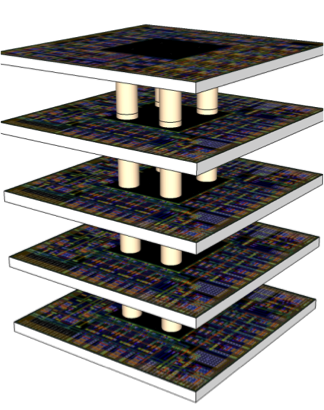
\includegraphics[width=0.2\columnwidth]{Plots/VIPRAM-3D.png}
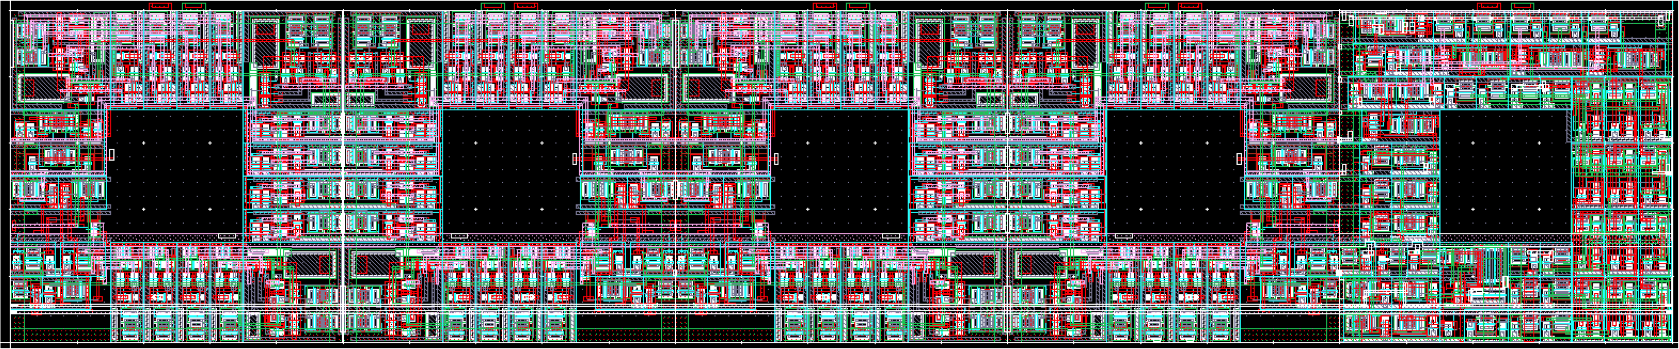
\includegraphics[width=0.3\columnwidth]{Plots/protoVIPRAM-2D.png}
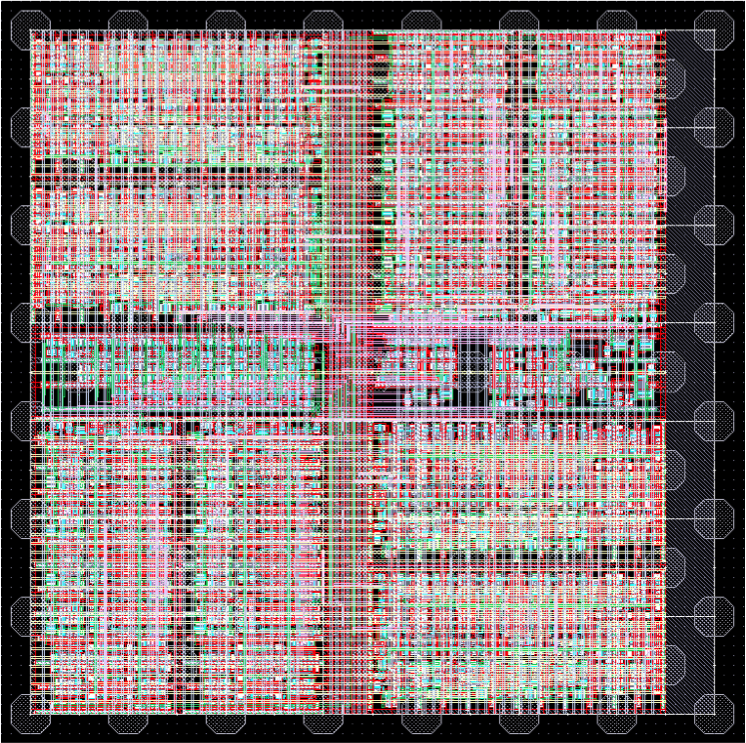
\includegraphics[width=0.2\columnwidth]{Plots/protoVIPRAM-L1CMS-pattern.png}
\caption{Left: We started with a 3D VIPRAM concept~\cite{bib:VIP-11} a few years ago and followed with a generic R\&D project~\cite{bib:VIP-12} funded by DOE CDRD.
Middle:  The first step taken was a 2D prototype (protoVIPRAM1) in which the associative memory building blocks were laid out in 2D as if this was a 3D design. A four layer AM pattern design in 130 nm for protoVIPRAM1, with a layout footprint of 25um X 125um size.
Room was left in the middle for as yet non-existent Through Silicon Vias and routing was performed to avoid these areas.
Right: One full eight layer AM pattern design in 130 nm for protoVIPRAM-L1CMS, with 70um x 70um size. Note there is no room left for TSVs in this case. One can then tile these pattern blocks on one tier uniformally, and have readout of fired roads on the second tier. The two tiers can be connected either via conventional bump bonding, or using the 3D DBI technology. Current plan is to have the design compatible with both approaches.}
\label{fig:protoVIPRAM-L1CMS-pattern}
\end{figure}

Both designs are in progress in CY2014 and will continue into CY2015, with chip submission expected in CY2015. Both designs will be on the same MPW run. To realize substantial savings in fabrication costs, protoVIPRAM-L1CMS will share wafer space with two additional chips being developed at Fermilab. One is our own protoVIPRAM3D, the other is the VIPIC (Vertically Integrated Photon Imaging Chip) designed to address the challenges of X-ray Correlation Spectroscopy (XCS). The VIPIC project is funded by BES.
Figure~\ref{fig:VIPRAM-MPW} shows the division 2:1:2 (area ratio) of a reticle between the protoVIPRAM-L1CMS (HEP/CMS), protoVIPRAM3D (HEP) and VIPIC (BES) projects on the planned 3D run. The total cost of the MPW is \$450K, and protoVIPRAM-L1CMS share is \$180K while the protoVIPRAM3D is \$90K. The protoVIPRAM3D work is supported by generic R\&D funds so far. 
The processing cost following the wafer stage is \$80K for protoVIPRAM-L1CMS, bringing the total cost to \$260K. We are requesting USCMS funds to cover the cost for protoVIPRAM-L1CMS.

\begin{figure}[ht!]
\centering
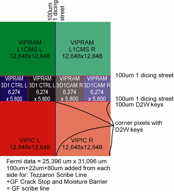
\includegraphics[width=0.35\columnwidth]{Plots/VIPRAM-MPW.png}
\caption{A drawing showing the division of a reticle between the VIPRAM (HEP) and VIPIC (BES) projects on the planned 3D run.
}
\label{fig:VIPRAM-MPW}
\end{figure}




\paragraph{Fermilab URA fellowships for VIPRAM R\&D and engineering students}

Last year, one URA fellowship was awarded to SMU Electrical Engineering graduate student for one year to work on the power and thermal analysis of the protoVIPRAM design. The work done by the student (from Prof. Ping Gui's group) 
has laid the foundation for the power and thermal analysis of the chip. This year another URA fellowship was awarded to Northwestern Electrical Engineering graduate student (from Prof. Seda Memik's group) to continue this work for one more year, this time with an emphasis on the protoVIPRAM3D power and thermal analysis. In addition, one visiting engineering student from BIST/India worked on
VIPRAM project for more than one year with extensive simulation and testing work done for the VIPRAM project.
This work was supported by generic R\&D funding. Over the past year, there has been three engneering master degree theses on VIPRAM. 

\paragraph{Work done by the Northwestern group}

The Northwestern group (lead by K. Hahn) has made significant progress over the past year on key aspects of system integration and data formatting/transfer.  Their integration efforts include the development of IPBus firmware and software for the Pulsar II based ATCA platform.  IPBus is a flexible, scalable application layer protocol that will become the primary means of DAQ/trigger slow control in Phase-2.  The group has developed a functioning implementation of IPBus firmware for both the Pulsar 2a and 2b, and has demonstrated control of Pulsar hardware with IPBus routed through a commercial ATCA switch.  The group's IPBus implementation is an important milestone for the AM-based Tracking Trigger project, and has facilitated the testing of AM prototypes at FNAL.

Northwestern is additionally developing and testing firmware that will integrate the Pulsar platform with the CMS/LHC TCDS system.  The firmware enables the Pulsar to receive LHC signals and clock and to distribute these within the ATCA shelf.  The team has successfully tested a basic version of the firmware with a $\mu\rm TCA$ GLIB and a legacy TTC system at CERN.  Their effort is now focused on transitioning the firmware to the Pulsar hardware.  A demonstration of TTC distribution over ATCA will be jointly conducted by Northwestern and FNAL at CERN in the near future.

With regard to data transfer, the Northwestern group is performing an extensive evaluation of the Aurora family of protocols from Xilinx.  These protocols are an industry-standard for low-latency, multi-gigabit serial communication.  The team is assessing the suitability of Aurora for application in the L1 trigger environment by simultaneously characterizing link latency and signal integrity.  Northwestern has shown that the Aurora 8b/10b protocol can be used to achieve $\sim130\rm~ns$ latency for point-to-point Pulsar communication over the ATCA backplane (Figure~\ref{fig:scope}).  The team has recently embedded a microblaze soft-processor in their Aurora test-bench to enable the in-system collection of link quality statistics as a function of transceiver/protocol configuration.


%-----------------------------------------------------------------
\begin{figure}[h]
\begin{center}
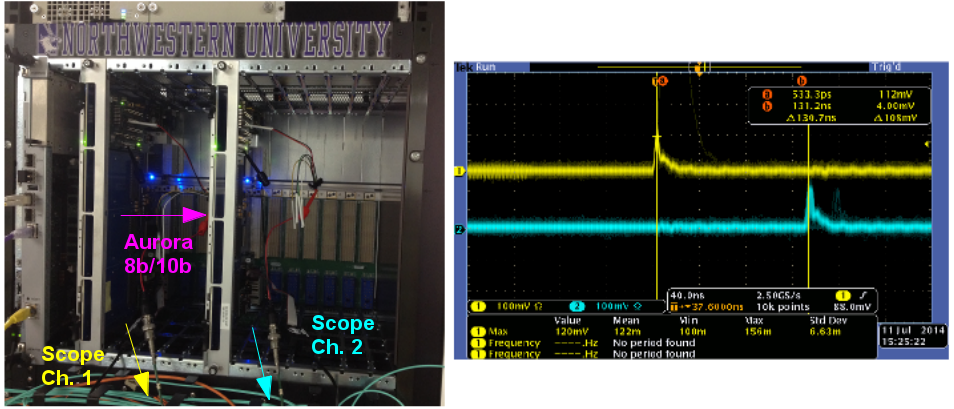
\includegraphics[width=0.80\linewidth]{Plots/crate_and_scope.png}
\caption{Left: Northwestern ATCA test-stand configured for Aurora link testing.  Right: scope trace showing $\sim 130\rm~ns$ latency for Aurora 8b/10b Pulsar-to-Pulsar communication over the ATCA backplane.}
\label{fig:scope}
\end{center}
\end{figure}
%-----------------------------------------------------------------

Northwestern has designed and proposed a data formatting scheme for the communication of stubs from the Tracker front-end to and within the Pulsar II ATCA-based trigger towers.  The proposed format was recently endorsed by the Tracker DAQ, Electronics and Tracking Trigger groups.  Northwestern (working closely with FNAL) is now developing a first firmware implementation of the corresponding data formatting pipeline for the Pulsar. Northwestern's work has been performed with Xilinx evaluation kits and two ATCA test-stands (one at the university and another at the Tracker Integration Facility at CERN) that the group has established.  To date, all equipment, IP licensing and personnel support for Northwestern's work has been privately funded.

The Northwestern group requests \$70K to hire a firmware engineer to support their on-going integration and development activities.  Hahn has a commitment from the University for an additional \$70K in matched funds for this purpose.  The combined funds will be sufficient to support a qualified junior engineer for 1-1.5 years.  The engineer will be based at Fermilab, which will facilitate the coordination and integration of his/her work with that of the overall project.

Northwestern also requests 12 months of COLA at \$1K per month for CERN-based postdoc Kevin Sung.  Kevin built and is responsible for the Northwestern test-stand at CERN.  This system is an important ``beachhead'' for the project at the lab.  The test-stand is located in the TIF next to a legacy TTC system, and thus has naturally become the center of the project's TTC integration efforts.  Soon, a new $\mu TCA$ CMS TCDS crate will also be installed at the TIF, and the Northwestern test-stand will be employed for integration testing with that system.  The CERN-based test-stand includes a $\mu TCA$ shelf, which provides a means of interface testing and development with Phase-2 Tracker FED prototypes.  As with the legacy systems, we anticipate that most of the hardware and operational expertise for the new TCDS and Tracker DAQ systems will be concentrated at CERN.



\paragraph{AM Simulaiton Work by USCMS}

Due to the intrinsic massively parallel processing nature of the AM operation, there is a clear challenge in using software based simulation to emulate the hardware performance and to aid its design. Here we are attempting to simulate the hundreds of million-fold parallelism of the L1 tracking trigger system (a non-von Neumann machine) with commercial CPUs (von Neumann machines).
Significant simulation preparation work has been done witin CMS in FY2014~\cite{bib:AM-CAMP}, and extensive simulation work is expected to be done in FY2015 in order to properly specify the demonstration system.  Fermilab/LPC/USCMS have been active in this area and will beome more heavily involved in the simulation efforts in FY2015. In particular, the Florida group (working closely with the Fermilab group through LPC) has a dedicated effort that attempts to significantly improve the performance of the simulation tool.
Three new groups have joined the project recently, TAMU, Rutgers, and UIC, and each plans to involve themselves in the simulation effort.

The existing simulation tools have been developed by different groups at various times. While they do provide a framework to perform studies, there are lots of room for improvement, specifially with regard to the memory required to simulate the AM hardware and the time required to generate test tracks. Improvement in the software would facilitate a dramatic improvement in how quickly the performance of the system can be studied and tested. This increase in efficiency would affect nearly all aspects of the project development. For this reason, a new software professional hire (with funding at 50\% FTE) is requested by both TAMU and Florida groups to stength the USCMS effort in this area. This would enable USCMS to drive the systematic evaluation of the performance requirements of the project. This work will optimize the number of roads required from the AM hardware, the data volumes and data links that must be handled, and the tracking performance requirements for physics output. The link between the hardware specifications from the tracker and AM to the physics performance requirements involves many tradeoffs that must be studied in a systematic way, with an understanding of the required trigger latencies and project cost. 


